\documentclass{article}

\usepackage{array}
\usepackage{longtable}
\usepackage{units}
\usepackage{booktabs}
\usepackage{graphicx}
\usepackage{amsmath, amsthm, amssymb, bm}
\usepackage{tikz, pgfplots}
\usetikzlibrary {shapes ,arrows , positioning }
\usetikzlibrary{calc,arrows.meta,positioning}
\usetikzlibrary{calc, automata, chains, arrows.meta}
\tikzset{
    every node/.style={font=\sffamily\small},
    main node/.style={thick,circle,draw,font=\sffamily\Large}
}
\usepackage{lipsum}
\usepackage{mwe}
\usetikzlibrary{shapes, arrows, positioning, fit, calc}
\newtheorem{theorem}{Theorem}
\newtheorem{Property}{Property}
\theoremstyle{remark}
\newtheorem*{defn}{Definition}
\renewcommand{\vec}[1]{\underline{#1}}
\usepackage{units}
\usepackage{fancyvrb}
\usepackage{hyperref}
\fvset{fontsize=\normalsize}

\title{AI1103 Assignement 7}
\author{Hritik Sarkar}

\newcommand\numberthis{\addtocounter{equation}{1}\tag{\theequation}}
\newcommand\inv[1]{#1\raisebox{1.15ex}{$\scriptscriptstyle-\!1$}}

\begin{document}
\maketitle
Paper - \href{https://csirhrdg.res.in/SiteContent/ManagedContent/ContentFiles/20190710103539182mathA_Dec2017.pdf}{Dec 2017-UGC-NET}
\\
Q120. Consider an M/M/1 queue with inter-arrival time having exponential distribution with mean $\frac{1}{\lambda}$ and service time having exponential distribution with mean $\frac{1}{\mu}$. Which of the following are true ?
\\1. if $0<\lambda<\mu$ then the queue length has limiting distribution Poisson~$(\mu-\lambda)$
\\2. if $0<\mu<\lambda$ then the queue length has limiting distribution Poisson~$(\lambda-\mu)$
\\3. if $0<\lambda<\mu$ then the queue length has limiting distribution which is geometric
\\4. if $0<\mu<\lambda$ then the queue length has limiting distribution which is geometric
\newline
\newline
Ans.
    The inter-arrival times are exponentially distributed with rate $\lambda$ implies that the arrival times are from Poisson distribution with parameter $\lambda$. The proof is given below.
    \newline
    
    Assume that the arrival times are from Poisson distribution with rate $\lambda$. Let $X_1$ is the time of first arrival. Then,
    \begin{align*}
        P(X_1 > t) &=  P(0\: arrival\: in \:(0,t])\\
        &= \frac{e^{-\lambda t}(\lambda t)^0}{0!}\\
        &=e^{-\lambda t}
    \end{align*}
    So,
    \[
    P(X_1\le t)=
    \begin{cases}
    1-e^{-\lambda t} \; when\;t>0 \\
    0 \; otherwise
    \end{cases}
    \]. This is the cdf of exponential distribution.
    So, $X_1\sim Exponential(\lambda)$.
\newline
\\
\\
This problem represents a continuous time infinite length markov chain, where each state represents the no. of persons in the queue. If a new person arrives, the state increases by one and if service for the first person in the queue is complete, he leaves and thus the state decreases by one. The chain is shown below
\\

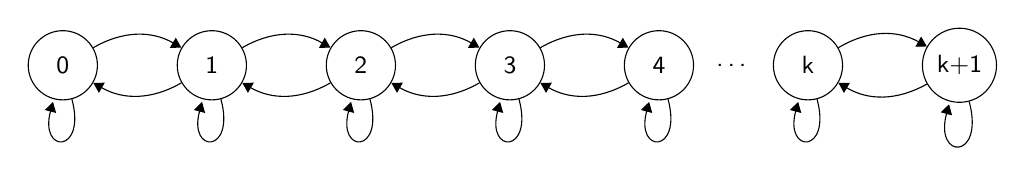
\begin{tikzpicture}[start chain = going right,
  -Triangle, every loop/.append style = {-Triangle}]
  \foreach \i in {0,...,4} 
    \node[state, on chain]  (\i) {\i};
  
  \foreach \i in {0,...,3} {
    \draw let \n1 = { int(\i+1) } in
      (\i)  edge[bend left] (\n1)
      (\n1) edge[bend left] (\i);
  }
  \foreach \i in {1,...,3}
    \draw  (\i) edge[loop below] (\i);
  \draw    (0)  edge[loop below]   (0);
  \draw    (4)  edge[loop below]  (4);
  
  \node [state , on chain] (k) {k};
  \node [state , on chain] (k+1) {k+1};
  \path (4) -- node[auto=false]{\ldots} (k);
  \draw (k) edge[bend left] (k+1);
  \draw (k+1) edge[bend left] (k);
  \draw (k) edge[loop below] (k);
  \draw (k+1) edge[loop below] (k+1);
  \end{tikzpicture}
Now, we have to find the transition probabilities. Since this is continuous time chain, the transition matrix at a particular time does not make much sense because we have to define it for any arbitrary time (time interval), instead we talk about it's derivative.\\
\newline
Consider, $P(t)$ is the infinite length row vector, in which each element represents the probability of being in that state (i.e. probability that the queue length is that value).
\[
    \frac{d\;P(t)}{dt}  = \lim_{{\delta t} \to 0} \frac{P(t+\delta t)-P(t)}{\delta t}
\]
For a discrete markov chain, Chapman-Kolmogorov property states that m+n step transition matrix = m step transition matrix $\times$ n step transition matrix. It's continuous analogous can be applied to simplify the above expression.
\begin{align*}
    \frac{d\;P(t)}{dt}  &= \lim_{{\delta t} \to 0} \frac{P(t+\delta t)-P(t)}{\delta t}\\
    &= \lim_{{\delta t} \to 0} \frac{P(t)\:P(\delta t)-P(t)}{\delta t}\\
    &= \lim_{{\delta t} \to 0} \frac{P(t)\:(P(\delta t)-\mathbb{I})}{\delta t}\\
    &= P(t) \lim_{{\delta t} \to 0} \frac{P(\delta t)-\mathbb{I}}{\delta t}\\
    &= P(t)\:Q
\end{align*}
where, $Q=\lim_{{\delta t} \to 0}\frac{P(\delta t)-\mathbb{I}}{\delta t}$ is called the jump-rate matrix.
\[
    \frac{d\;P(t)}{dt} = P(t)\:Q
\]
In case there exists a limiting distribution we need to solve $\frac{d\;P(t)}{dt}=0$. Equivalently we can say, we need find a non-zero vector $\pi$ such that $\pi Q = 0$.
Now, Poisson arrival means,
\[
    \lim_{{\delta t} \to 0} \frac{P_{k\:k+1}(\delta t)}{\delta t} = \lambda
\]
exponential service time means,
\[
    \lim_{{\delta t} \to 0} \frac{P_{k\:k-1}(\delta t)}{\delta t} = \mu
\]
Now,
\begin{align*}
    \lim_{{\delta t} \to 0} \frac{P_{k\:k}(\delta t)}{\delta t} &=  \frac{1-P_{k\:k+1}-k\:k-1}{\delta t}\\
    &= -\mu-\lambda+\lim_{{\delta t} \to 0} \frac{1}{\delta t}
\end{align*}
Now, we can define the jump rate matrix as follows,
\begin{align*}
    Q = \lim_{{\delta t} \to 0} \frac{P(\delta t)-\mathbb{I}}{\delta t} = 
\begin{pmatrix}
-\lambda & \lambda & 0 & \cdots \\ 
 \mu& -\mu-\lambda & \lambda & \cdots \\ 
 0 & \mu & -\mu-\lambda & \cdots \\ 
 \vdots & \vdots & \vdots & \ddots 
\end{pmatrix}
\end{align*}
Now, we can try to find the limiting distribution by trying to find a non-zero $\pi$ such that, $\pi\:Q=0$.
\[
    \pi = 
    \begin{bmatrix}
 \pi_0& \pi_1& \pi_2 & \pi_3 & \pi_4 & \cdots 
\end{bmatrix}
\]
This is equivalent of solving the the following difference equation-
\[
    \lambda \pi_k - (\mu+\lambda) \pi_{k+1} + \mu \pi_{k+2} = 0 \numberthis{\label{1}}
\]
with $\pi_0=\pi_0$ and $\pi_1=\frac{\lambda}{\mu}\pi_0$
Taking z-transform on the both sides of \eqref{1} and using the shifting-property of z-transform,
\begin{align*}
    \lambda \pi(z) - (\mu+\lambda) z \left [\pi(z)-\pi_0 \right ]+ \mu z^2 \left [ \pi(z)-\pi_0-\frac{\lambda}{\mu}\frac{\pi_0}{z} \right ] = 0
\end{align*}
\begin{align*}
    \pi(z) \left [ \lambda - (\mu+\lambda) z + \mu z^2  \right ] = - (\mu+\lambda) z \pi_0 + \mu z^2 \pi_0 + \lambda \pi_0 z
\end{align*}

\begin{align*}
    \pi(z) \left [ \lambda - (\mu+\lambda) z + \mu z^2  \right ] = - (\mu+\lambda) z \pi_0 + \mu z^2 \pi_0 + \lambda \pi_0 z
\end{align*}
\begin{align*}
    \pi(z) = \frac {\pi_0 z (-\mu+\mu z)}{(\lambda-\mu z)(1-z)}
\end{align*}
\begin{align*}
    \pi(z) = \frac {\pi_0 z \mu }{(\mu z-\lambda)} 
\end{align*}
\begin{align*}
    \pi(z) = \frac {\pi_0 z}{(z-\frac{\lambda}{\mu})}
\end{align*}
taking the inverse z-transform we get,
\[
    \pi_k = \pi_0 \left ( \frac{\lambda}{\mu} \right )^k
\]
Since $\pi$ is a vector of probabilities, the sum of all should be 1.
So,
\[
    \pi_0 + \pi_1 + \pi_2 + \pi_3 + + \pi_4 + \cdots = 1 
\]
\[
    \pi_0 \left ( 1+ \left ( \frac{\lambda}{\mu} \right )^1 + \left ( \frac{\lambda}{\mu} \right )^2 + \left ( \frac{\lambda}{\mu} \right )^3 + + \left ( \frac{\lambda}{\mu} \right )^4 + \cdots \right) = 1
\]
\[
    \pi_0 \sum_{k=0}^{\infty} \left ( \frac{\lambda}{\mu} \right )^k = 1
\]
This is an infinite geometric series, and this will converge only if $\frac{\lambda}{\mu} < 1$
\[
    \pi_0 \left ( \frac{1}{1-\frac{\lambda}{\mu}} \right ) = 1
\]
\[
    \pi_0 = \left ( 1-\frac{\lambda}{\mu} \right )
\]
So,
\[
\pi_k = \left ( \frac{\lambda}{\mu} \right )^k \left (  1-\frac{\lambda}{\mu} \right )
\]
This represents geometric distribution with parameter $\left (  1-\frac{\lambda}{\mu} \right )$. (Ans.)
\newline
The condition $\frac{\lambda}{\mu} < 1$ or $\lambda<\mu$ does seem to be correct intuitively. In case the arrival rate $(\lambda)$ is more than service rate $(\mu)$ the queue will be of infinite length which won't have a stationary distribution.

\end{document}
